\documentclass[tikz,border=4pt]{standalone}
\usepackage{amsmath}
\begin{document}
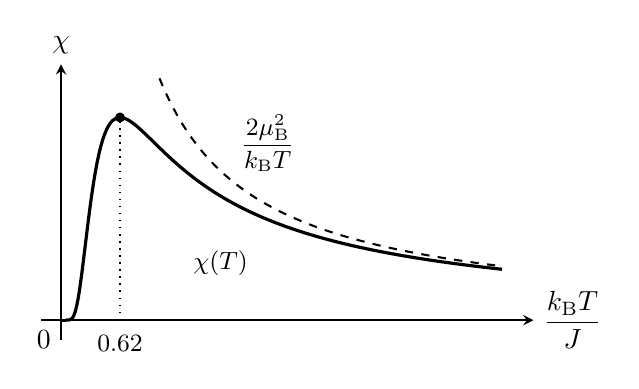
\begin{tikzpicture}[>=stealth, thick, scale=1.0]
  % Axes: x = k_B T / J from 0 to 4.8 (scale 1.2 cm per unit -> 5.76 cm)
  % y = chi * J / mu_B^2 from 0 to 1.61 (scale 1.6 cm per unit -> peak ~ 2.58 cm)
  \draw[->, line width=0.65pt] (-0.25, 0) -- (6.0, 0) node[right] {$\dfrac{k_{\mathrm{B}}T}{J}$};
  \draw[->, line width=0.65pt] (0, -0.25) -- (0, 3.25) node[above] {$\chi$};
  \node[below left] at (0, 0) {$0$};

  % Overflow-free exact 2-spin susceptibility:
  % f(t) = 8 * exp(-1/t) / (t * (1 + 3*exp(-1/t))), with t = x / 1.2
  \draw[line width=1.15pt, domain=0.06:5.6, samples=140, smooth]
    plot (\x, {1.6 * 8 * exp(-1.2/\x) / ((\x/1.2) * (1 + 3*exp(-1.2/\x)))});
  \draw[line width=1.15pt] (0, 0) -- (0.06, 0);

  % High-T Curie asymptote: 2 / t = 2.4 / x (dashed)
  \draw[dashed, line width=0.75pt, domain=1.25:5.6, samples=80, smooth]
    plot (\x, {1.6 * 2 / (\x/1.2)});

  % Peak marker at t = 0.624 (x = 0.749, y = 2.575)
  \draw[dotted, line width=0.55pt] (0.749, 0) -- (0.749, 2.575);
  \fill (0.749, 2.575) circle (1.8pt);
  \node[below, font=\small] at (0.749, -0.06) {$0.62$};

  % Labels for asymptotes
  \node[font=\small, right] at (2.15, 2.25) {$\dfrac{2\mu_{\mathrm{B}}^2}{k_{\mathrm{B}}T}$};
  \node[font=\small, right] at (1.55, 0.72) {$\chi(T)$};
\end{tikzpicture}
\end{document}
